\documentclass[conference]{IEEEtran}
\usepackage{graphicx}
\usepackage{amsmath}
\usepackage{booktabs}
\usepackage{array}
\usepackage[table]{xcolor}
\usepackage[hidelinks]{hyperref}
\usepackage{balance}

\graphicspath{{../figures/}}

\newcommand{\ugm}{$\mu$g/m$^3$}

\setlength{\textfloatsep}{9pt plus 2pt minus 3pt}
\setlength{\dbltextfloatsep}{9pt plus 2pt minus 3pt}

\begin{document}

\title{Exact Concept-Grouped SHAP Explanations of a Deployed Real-Time
PM2.5 Ensemble for Texas Census Tracts}

\author{
\IEEEauthorblockN{Nathan Tan}
\IEEEauthorblockA{St. Mark's School of Texas\\
Dallas, TX, USA\\
nathantan2027@gmail.com}
\and
\IEEEauthorblockN{Saketh Chebrolu}
\IEEEauthorblockA{St. Mark's School of Texas\\
Dallas, TX, USA\\
chebrolusaketh@gmail.com}
\and
\IEEEauthorblockN{Yifeng Wang}
\IEEEauthorblockA{School of Civil and Environmental Engineering\\
Georgia Institute of Technology\\
Atlanta, GA, USA\\
\colorbox{yellow}{[email pending]}}
}

\maketitle

\begin{abstract}
Low-cost sensor networks now support operational, neighborhood-scale air
quality tools, but the machine learning models behind these tools are rarely
explained to the communities that rely on them. We present the explanation
layer of Shared Skies, a deployed web platform that maps fine particulate
matter (PM2.5) in real time across all 6,896 Texas census tracts using a
tree ensemble trained on 285,798 daily readings from 310 PurpleAir sensors
and validated at a leave-one-sensor-out coefficient of determination of
0.71. Because SHAP attributions are additive and the deployed prediction is
a convex blend of tree models, blending per-model TreeExplainer
attributions with the deployment weights reproduces the ensemble output to
within one millionth of the measurement unit. Summing attributions within
seven concept groups yields a decomposition non-specialists can read in
physical units. The
explanations show that the model is chiefly a spatial nowcaster: features
describing nearby sensors dominate globally, carry a major smoke event
almost alone while the dedicated smoke tier adds at most 0.31 micrograms
per cubic meter, and actively suppress predictions during hyper-local events
that no neighboring sensor observes. We report guardrails for policy
interpretation, including inverted proximity features and strictly
correlational environmental justice attributions, and show how explained
failures motivate targeted sensor placement.
\end{abstract}

\begin{IEEEkeywords}
explainable artificial intelligence, SHAP, air quality, PM2.5, low-cost
sensors, ensemble learning, environmental monitoring
\end{IEEEkeywords}

\section{Introduction}
Low-cost optical sensors have changed who gets to see air pollution.
Networks such as PurpleAir now report fine particulate matter (PM2.5) at
neighborhood scale and minute cadence, and corrected versions of their data
now feed public tools such as the AirNow Fire and Smoke Map
\cite{barkjohn2021}. The
placement of these sensors is itself uneven across income groups
\cite{desouza2021}, so the models that interpolate between them are, for
many communities, the only air quality information available.

Such tools are judged almost entirely on accuracy. A fused ensemble over
sensor, satellite, meteorological, and demographic inputs can validate
well yet behave in ways its operators would not expect, and when its
outputs color a public map or steer monitor placement, unexamined behavior
is a liability. Shapley additive explanation
(SHAP) methods \cite{lundberg2017, lundberg2020} have made attribution
practical for tree models, and environmental applications such as
flood-susceptibility mapping have begun to adopt them \cite{choubin2025}.
Yet the
explanations almost always describe research models; deployed systems,
the ones people actually consult, remain largely unexplained.

This paper explains one such system exactly. Shared Skies is a live web
platform that predicts PM2.5 for every census tract in Texas from PurpleAir
sensors and public data streams, refreshing continuously. We contribute:
(1) an exact explanation layer for the deployed convex tree ensemble, which
blends per-model TreeExplainer attributions with the deployment weights to
reconstruct every pre-clipping output to within $10^{-6}$~\ugm{}, then
partitions the 38 features into seven concept groups so that each
prediction becomes a short physical story; (2) a characterization of what the deployed model actually
learned, which is dominated to a degree accuracy metrics never reveal by
same-day readings from neighboring sensors; and (3) an explanation-driven
failure analysis showing that the same neighbor features that produce the
model's accuracy actively suppress its predictions during hyper-local
pollution events, a structural blind spot that argues for targeted sensor
placement rather than model tuning.

\section{The Deployed System}
\subsection{Platform}
Shared Skies serves a public, bilingual web map of model-estimated 24-hour
PM2.5 for all 6,896 Texas census tracts. The backend pulls live PurpleAir
readings, cached for 15 minutes, recomputes the full feature set, runs the
ensemble for every tract, and caches predictions for 30 minutes. A served
value estimates a tract's daily-mean-equivalent PM2.5 given current
conditions; the training feature pipeline is reproduced at serving time, so
sub-daily dynamics enter only through the inputs. The tract color scale
breaks at 9~\ugm{}, adopting the level of the 2024 annual PM2.5 standard
\cite{epa2024naaqs} as a fixed reference for the 24-hour map. A second view
proposes future sensor placements, which Section~\ref{sec:discussion}
connects back to the explanations.

\subsection{Training data and features}
The training target is the daily mean of the raw PurpleAir ATM-channel
PM2.5 concentration. Readings are restricted to 0 to 200~\ugm{} and
cleaned per sensor with a robust z-score rule on median absolute
deviation; sensors with fewer than 60 valid days, near-constant output, or
medians indicating indoor placement are dropped. The result is 285,798 daily
readings from 310 outdoor sensors inside Texas between January 2021 and May
2026. Sensors in border states contribute same-day neighbor context but are
never training targets. The raw ATM channel is kept, rather than corrected
\cite{barkjohn2021}, so that training targets and live inference share
semantics; Section~\ref{sec:discussion} revisits this choice. Days with
means above 75~\ugm{} are excluded
from training, a choice whose consequences the explanations make visible.

Each row carries 38 features (Table~\ref{tab:groups}): daily weather from
Open-Meteo \cite{zippenfenig}; same-day neighbor statistics (mean and
count of other sensors within 25, 50, and 100~km, plus dispersion at
50~km, computed with a haversine BallTree); an ordinal smoke tier from
NOAA Hazard Mapping System (HMS) analyst polygons \cite{brey2018}; aerosol optical depth and surface PM2.5
from the Copernicus Atmosphere Monitoring Service (CAMS) \cite{peuch2022};
eight tract-level environmental justice indicators from EPA EJScreen
\cite{ejscreen}; location and distance covariates; and calendar encodings.

\subsection{Ensemble and validation}
Four regressors are trained: a random forest \cite{breiman2001}, LightGBM
\cite{ke2017}, XGBoost \cite{chen2016}, and CatBoost
\cite{prokhorenkova2018}. Validation is leave-one-sensor-out (LOSO): each of
the 310 sensors is held out in turn, models are refit on the rest, and,
critically, the neighbor features of every training row are recomputed with
the held-out sensor removed from the pool, closing a same-day leakage path
that random splits cannot detect. Spatially naive cross-validation is known
to overstate the skill of models like this one \cite{meyer2022}; under
random 80/20 splitting this ensemble scores $R^2=0.84$, which LOSO deflates
to 0.71.

Blend weights are a simplex-constrained convex combination fit on the LOSO
out-of-fold predictions and selected by a grouped cross-fit over sensors.
The deployed weights are 0.6827 (random forest), 0.3094 (CatBoost), 0.0079
(LightGBM), and exactly zero for XGBoost, giving LOSO $R^2=0.7136$ against
0.7114 for an equal-weight blend and an inverse-MSE baseline at 0.7126
(RMSE 4.22~\ugm{}, MAE 2.62~\ugm{}). The random forest alone reaches
0.7138: at this resolution the top candidates are tied, and the deployment
is a nearly single-model instance of the convex blends the method covers.
We explain the blend because the blend is what ships. Live inference
fills unavailable features with training medians.

\begin{table}[t]
\caption{The seven concept groups partitioning the 38 model features
(group sizes in parentheses).}
\label{tab:groups}
\centering
\footnotesize
\begin{tabular}{>{\raggedright\arraybackslash}p{0.30\columnwidth}>{\raggedright\arraybackslash}p{0.58\columnwidth}}
\toprule
Group & Features \\
\midrule
Regional PM signal (9) & neighbor PM2.5 mean and count at 25, 50, 100 km;
dispersion at 50 km; CAMS AOD; CAMS PM2.5 \\
Wildfire smoke (1) & HMS smoke tier (none/light/medium/heavy) \\
Meteorology (7) & temperature, humidity, pressure, wind speed,
precipitation, two interaction terms \\
Local sources (4) & EJScreen traffic, diesel PM, Superfund, and Risk
Management Plan facility proximity \\
Community and EJ context (4) & EJScreen demographic index; percent people
of color, low income, linguistically isolated \\
Geography (4) & latitude, longitude, distance to coast, distance to
nearest sensor \\
Season and calendar (9) & month, weekday, day of year, and their
sine/cosine encodings \\
\bottomrule
\end{tabular}
\end{table}

\section{Exact Ensemble Explanations}
\subsection{Blending per-model attributions}
The deployed prediction for features $x$ is
$f(x)=\max\bigl(0,\sum_m w_m f_m(x)\bigr)$ over the three models with
$w_m>0$. TreeExplainer \cite{lundberg2020} decomposes each tree model
exactly as $f_m(x)=b_m+\sum_j \phi^m_j(x)$. Attributions are additive, so

\begin{equation}
\sum_m w_m f_m(x) = b + \sum_j \phi_j(x)
\label{eq:blend}
\end{equation}

with $b=\sum_m w_m b_m$ and $\phi_j(x)=\sum_m w_m \phi^m_j(x)$ is an
additive decomposition of the pre-clipping ensemble output, computed
without sampling or surrogate models. Exact here means local accuracy,
faithful reconstruction of this model's output, not axiomatic Shapley
values under an interventional distribution: TreeExplainer (SHAP 0.50.0)
runs in tree-path-dependent mode, which conditions on the training
distribution through tree cover counts, and its credit assignment among
correlated features differs from interventional variants. The audit of
Eq.~\eqref{eq:blend} runs wherever rows are explained; over the 6,000-row
global sample the maximum absolute reconstruction error is
$8.9\times10^{-7}$~\ugm{} (mean $5.9\times10^{-8}$); the residual reflects
float32 caching, and direct float64 explanation of individual rows
reconstructs to $5\times10^{-13}$~\ugm{}. The serving layer applies only a
final clip at zero, which never binds on the sampled predictions (minimum
raw output $+0.4$~\ugm{}).

\subsection{Concept groups}
Individual attributions for 38 features are exact but not legible to a
public audience. We therefore partition the features into the seven concept
groups of Table~\ref{tab:groups} and report group sums
$\Phi_G(x)=\sum_{j\in G}\phi_j(x)$. Because the partition is exhaustive and
disjoint, $b+\sum_G \Phi_G(x)$ still reconstructs the prediction exactly;
runtime validation asserts the partition against the deployed feature list.
Note that a group's global importance, the mean absolute summed
contribution, falls below the sum of member importances when members
cancel.

\subsection{Analysis protocol}
Global structure is computed over a uniform 6,000-row sample of the training
frame (seed 42). Feature response is analyzed with dependence scatters,
12-quantile binned medians, and Spearman rank correlations between feature
value and attribution, with bootstrap intervals clustered by sensor. Because the sample contains only five heavy-smoke
rows, tier-level smoke statistics are recomputed exactly over all 431
heavy-tier rows in the corpus and a 2,500-row sample of the medium tier,
with 2,000-resample percentile-bootstrap 95\% confidence intervals. Two
full days are explained
sensor-by-sensor: the strongest smoke day (May 27, 2024) and the cleanest
day (April 3, 2024) among days with at least 150 reporting sensors. Local
cases follow fixed rules: the highest-reading smoke-day row predicted
within 35\% of its observation, and the worst underprediction above
40~\ugm{}. All pipeline outputs reproduce byte-identically, and every
analysis number in this paper is regenerated by verification scripts
released with the code.

\begin{figure}[t]
\centering
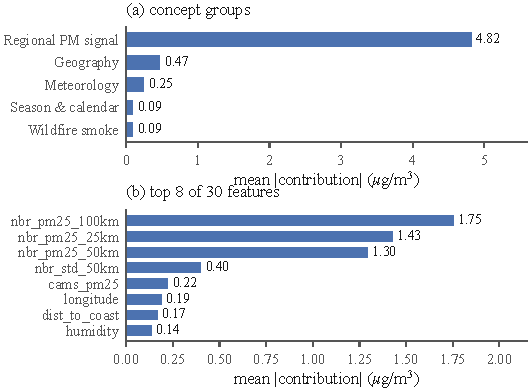
\includegraphics[width=\columnwidth]{fig2_global}
\caption{Global importance over the 6,000-row sample. (a) Mean absolute
concept-group contribution; the regional PM signal exceeds every other
group by an order of magnitude. (b) The top individual features are the
three neighbor means, neighbor dispersion, and CAMS surface PM2.5.}
\label{fig:global}
\end{figure}

\section{Results}
\subsection{The model is a spatial nowcaster}
Fig.~\ref{fig:global} shows global importance. The regional PM signal group
averages 4.84~\ugm{} of absolute contribution per prediction; the next
group, community and EJ context, averages 0.39~\ugm{}, and the dedicated
smoke tier is last at 0.05~\ugm{}. The three neighbor-mean
features are individually the three most important inputs (1.86, 1.37, and
1.36~\ugm{} at 100, 50, and 25~km). Whatever else the ensemble encodes, its
predictions are first and foremost a spatial average of what nearby sensors
already report. The ordering is robust: a sensor-clustered bootstrap
reproduces the full group ranking in 89.3\% of 1,000 resamples, and grouped
permutation importance orders the seven groups identically (rank
correlation 1.0).

\subsection{Feature response and semantics}
Dependence analysis (Fig.~\ref{fig:dependence}) sharpens this picture in
five ways.

\subsubsection{Near-linear regional response} The 50~km neighbor mean maps
onto its attribution almost monotonically (Spearman $\rho=0.994$), with
slope 0.26~\ugm{} per 1~\ugm{} of neighbor mean below 30~\ugm{}, then
flattens: recomputed exactly over the corpus, the median contribution is
$+6.3$~\ugm{} for neighbor means between 30 and 40~\ugm{} and $+8.0$~\ugm{}
(CI $[7.93, 7.97]$, all 860 qualifying rows) above 40~\ugm{}. The
flattening is consistent with the exclusion of training days above
75~\ugm{}: the model has little headroom to extrapolate events it never
saw.

\subsubsection{The smoke tier is nearly redundant, and not monotone} Mean
attribution of the HMS tier, in \ugm{}, is $-0.044$ (none) and $+0.060$
(light) on the sample, $+0.110$ over 2,500 recomputed medium-tier rows
(CI $[0.108, 0.111]$), and $+0.097$ over all 431 heavy-tier rows
(CI $[0.094, 0.101]$). Heavy plumes contribute less than medium ones
(bootstrap difference CI $[0.008, 0.016]$~\ugm{}), though the
$0.012$~\ugm{} gap is negligible against an RMSE of 4.22. Only 431 of
285,798 training rows (0.15\%) carry the heavy tier, and on those rows mean
observed PM2.5 is lower than on medium-tier rows (11.6 versus
16.6~\ugm{}), a reminder that an analyst-drawn plume overhead does not
guarantee surface-level smoke. The model nearly ignores a feature whose
evidential value its training data did not support.

\subsubsection{Proximity features invert at the extreme} Traffic proximity
attribution is flat over most of its range, then turns negative past
roughly the 85th percentile: mean $-0.36$~\ugm{} beyond that point,
$-1.15$~\ugm{} over the top two percent, and single predictions as low as
$-3.6$~\ugm{}. Diesel PM proximity behaves the same way at smaller
magnitude. Extreme proximity marks dense urban cores whose sensor-rich
surroundings already carry the level; the model uses it as a downward
geographic correction, not an emissions signal. A naive
reading, that traffic lowers pollution, would invert the causal reality.

\subsubsection{EJ context is small, monotone in binned median, and
strictly correlational}
Attribution rises with percent linguistically isolated ($\rho=0.622$,
sensor-clustered bootstrap CI $[0.52, 0.72]$) and percent people of color
($\rho=0.628$, CI $[0.53, 0.72]$); above its 70th percentile, linguistic
isolation is associated with binned-median attributions of up to
$+0.49$~\ugm{}. These are learned
associations between demographics and measured PM2.5 under the model's
other inputs. They must never be presented as demographic causation, and
we do not compute counterfactuals over them.

\subsubsection{Interactions stay inside the regional group} SHAP
interaction values (a 300-row subsample, seed 42; random forest and
CatBoost combined with renormalized weights covering 99.2\% of the blend,
LightGBM at weight 0.008 omitted) rank every leading pair
within the regional signal group: the neighbor means interact at 0.50,
0.46, and 0.28~\ugm{} mean absolute strength, followed by
neighbor-dispersion pairs. The strongest pair that crosses group lines,
diesel proximity with linguistic isolation, is an order of magnitude
weaker at 0.05~\ugm{}. Regional dominance is not an artifact of additive
attribution.

\begin{figure*}[t]
\centering

\includegraphics[width=\textwidth]{fig3_dependence}
\caption{Feature dependence on the 6,000-row sample (gray points; blue line
is the 12-quantile binned median). (a) Contribution of the 50 km neighbor
mean is near-linear then flattens above 40~\ugm{}. (b) HMS smoke tier:
red markers are exact means over all 431 heavy-tier rows and 2,500
medium-tier rows with bootstrap 95\% intervals; heavy contributes less than
medium. (c) Traffic proximity is inert until roughly the 85th percentile,
then turns negative. (d) Linguistic isolation rises monotonically past its
70th percentile.}
\label{fig:dependence}
\end{figure*}

\begin{figure}[t]
\centering

\includegraphics[width=\columnwidth]{fig4_event_maps}
\caption{Every reporting sensor explained on the strongest smoke day
(top, 156 sensors, 98.7\% under a plume) and the cleanest day (bottom, 154
sensors): regional-signal contribution (left) and predicted PM2.5 (right).
The event is carried almost entirely by the regional signal
($+24.8$~\ugm{} statewide mean) while the smoke tier never exceeds
$+0.31$~\ugm{} anywhere in the state.}
\label{fig:maps}
\end{figure}

\subsection{Two days, one mechanism}
On May 27, 2024
(Fig.~\ref{fig:maps}), with 98.7\% of sensors under an analyst-drawn plume
and a statewide mean reading of 37.0~\ugm{}, the model predicts a mean of
36.1~\ugm{}, and the regional signal group contributes $+24.8$~\ugm{} of
that on average. The smoke tier's largest contribution anywhere in the
state is $+0.31$~\ugm{}. On April 3, 2024 (statewide mean 1.03~\ugm{}), the
regional group pulls predictions down by 7.6~\ugm{} on average from the
9.72~\ugm{} baseline. Smoke information reaches the model through the
neighbor network, not the smoke feature: both days are settings of one
nowcasting mechanism.

\subsection{Explaining a success and a failure}
Fig.~\ref{fig:cases} decomposes two individual predictions. On the smoke
day, sensor 217461 read 71.1~\ugm{} and the model predicted 49.6~\ugm{},
with $+34.6$~\ugm{} from the regional signal and $+0.29$~\ugm{} from the
smoke tier; even this detection underpredicts, consistent with the
capped training range and the saturating neighbor response. On November 19,
2024, sensor 242357 read 75.0~\ugm{}, at the retention boundary itself,
while every neighbor mean sat below 1.8~\ugm{}; the model predicted
6.2~\ugm{}. The explanation shows why: the regional group contributed
$-6.1$~\ugm{}, the three neighbor means $-2.5$ to $-1.7$~\ugm{} each. Nor
is the case unique: 46 corpus rows read at least 40~\ugm{} with every
neighbor mean below 5~\ugm{}; the regional group is negative on all 46
(mean $-5.2$~\ugm{}), and the highest prediction among them is 9.1~\ugm{}
against a mean observation of 54.1~\ugm{}. Rows above 75~\ugm{} were
excluded (241 pre-cap), so these figures lower-bound the blind spot. The
features that make the model accurate on regional events actively vote
against hyper-local ones; no reweighting of the same features can fix what
the network cannot see.

\begin{figure}[t]
\centering

\includegraphics[width=\columnwidth]{fig5_cases}
\caption{Exact concept-group decomposition of two predictions. (a) A
detected smoke event is carried by the regional signal; the smoke tier
adds $+0.3$~\ugm{}. (b) The worst miss in the corpus: neighbors saw
nothing, and the regional signal suppresses the prediction below the
baseline.}
\label{fig:cases}
\end{figure}

\section{Discussion}
\label{sec:discussion}

\subsection{For model builders} The smoke tier could be replaced, not
retuned: candidate representations include plume density, smoke age, or
lagged fire radiative power; only 431 heavy-tier rows support the current
one. The saturating neighbor
response ties directly to the 75~\ugm{} training cap, so raising the cap
(or modeling exceedances separately) is a measurable next experiment.

\subsection{For network operators} The miss case turns an error metric
into a map, with one caution: sign alone cannot separate clean
surroundings from unsensed ones (the clean day's statewide mean,
$-7.6$~\ugm{}, is as negative as El Paso's annual $-7.0$~\ugm{}). Sparsity
separates them: the El Paso sensor averages 0.8 same-day neighbors within
50~km against a statewide 27, while densely sensed East Texas runs
$+9.3$~\ugm{}. Persistently negative regional means in sparse
neighborhoods mark where predictions rest on remote evidence (distance to
the nearest sensor reaches 164~km), and those are the places where the
platform's placement optimizer should spend new sensors; the explanation
layer supplies that prioritization for free.

\subsection{For communicating attributions} SHAP explains the model, not
the atmosphere. The traffic inversion shows a raw attribution
contradicting physical causality; the EJ attributions show a small,
systematic association that could be misread causally. Any deployment
of these explanations to a public dashboard needs the concept-group
framing, the correlational disclaimer, and suppression of counterfactuals
on demographic features as defaults, not footnotes.

\subsection{Limitations} The target is the uncorrected ATM channel, so
absolute levels are not comparable to regulatory monitors without a
correction such as that of Barkjohn et al. \cite{barkjohn2021}; the
explanations inherit whatever bias that channel carries. Days above
75~\ugm{} are absent from training, so extreme-event behavior describes a
model that never saw the worst days, and the failure analysis lower-bounds
the blind spot. LOSO $R^2$ characterizes held-out sensor locations;
accuracy at unsensed tracts is unquantified, and the miss case suggests it
degrades exactly there. The EJ attributions are further conditioned on a
network whose placement is itself demographically uneven
\cite{desouza2021}, so their sign and size partly reflect where sensors
exist. Tree-path-dependent attribution spreads credit among correlated
features, so within-group rankings are less certain than group totals. Explanation statistics describe the training frame, not the
serving distribution. The findings describe one model over one state and
five years; the method applies unchanged to any convex blend of tree
models.

\section{Conclusion}
We converted a deployed, accuracy-validated PM2.5 mapping system into one
whose every prediction can be read: an exact blend of per-model
TreeExplainer attributions, folded into seven concept groups, reconstructs
each output to within $10^{-6}$~\ugm{}. The reading is unflattering in
places. The model is a spatial nowcaster that nearly ignores its smoke
flag, inverts proximity features at the urban extreme, and structurally
cannot see events its sensor network does not cover. None of this is
visible in $R^2$, and all of it matters for how the tool should be used,
improved, and communicated. Explaining 6,000 predictions takes 20 minutes
on a desktop CPU and one prediction a fraction of a second, so attaching
exact, plainly narrated explanations to the live platform is the immediate
next step.

\balance
\bibliographystyle{IEEEtran}
\bibliography{../references}

\end{document}
